\chapter{Analysis} \label{analysis}

When assembling a multifunctional, reusable toolkit, it is crucial to map the exact user needs.
The following chapter analyses the user requirements and project use cases. 
It also describes different user roles and states general functional and nonfunctional requirements for the software.

% Despite the fact that this work encompasses creating a comprehensible web automation definition format, an interpreter of this format and an \ac{GUI} editor, 
% there is no point in carrying out user analysis for the format itself, since it only specifies the grammar of the definition file. 

% Therefore, the following sections conduct the analysis only for the \ac{SW} part of the work, i.e. the interpreter and the editor.

\section{User roles} \label{userroles}

In the first section of the analysis, we describe the typical users of such a toolkit.
Users may have different requirements based on their level of expertise and knowledge.
While the toolkit should be accessible and user-friendly enough to allow beginners to
create web automations with ease, it also should provide the more experienced users with 
advanced functionality required for handling specific use cases. 

For clarity, we describe only two user roles with a significant difference in skill and knowledge.
Please note that these roles are rather exemplatory and do not describe actual users the author has met.
Their main purpose is to provide a clear dichotomy between two common groups of \acl{SW} users.

\subsection{User} \label{UserUserRole}
\textit{User} has a fairly basic knowledge of using personal computers 
and web-related technologies - knowledge of e.g. \textit{CSS} or \textit{XPath} selectors is expected.
A \textit{User} wants to reach their goal without much additional knowledge and/or specialized tools.

Such a user wants to use the toolkit in the most basic way.
While they might have some experience with the technologies used in the toolkit, they generally do not want to use the toolkit programmatically and rely on the \ac{GUI} tools only.

Their automation use case is easily described, mostly as a linear sequence of well-defined, simple steps.
Some examples of such use cases might be \textit{automated data extraction} and simple \textit{\acl{RPA}}.


\subsection{Developer} \label{DevUserRole}
The \textit{Developer} user role describes an intermediate-to-expert computer specialist with deep
knowledge of computer systems, programming and web-related technologies.
This user role expects to take advantage of the advanced features of the toolkit, possibly spending some extra time learning how to use those properly.

They might not want not only to create and run automations but also to use the toolkit programmatically, 
install the toolkit components on their systems or edit parts of the toolkit. 

When creating an automation, the \textit{Developer} has more complicated use cases with possibly branching scenarios. 
Those might be more \textit{elaborate data extraction} cases, \textit{software testing}, \textit{complicated \ac{RPA}} and other.

\section{Requirements}
\label{requirements}

The following section describes functional and non-functional requirements for the toolkit project, 
based on the requirements of the user roles described in the \autoref{userroles} User roles.

For clarity, let us divide the toolkit project into individual tools serving different purposes.
As the main purposes of the toolkit are \textit{creating}, \textit{editing} and \textit{running web automations},
we can talk about the \textit{Editor} and the \textit{Runner} parts separately.

\emptyline
\subsection{Editor}

The \textit{Editor} is the part of the toolkit allowing the users to create and edit the web automations.
It should provide a user-friendly way of doing so while not restricting the more advanced users.

The ultimate goal of the \textit{Editor} is not to exhaustively support all the features of the workflow definition syntax but to provide a simple and intuitive way of creating and editing web automations.

\smallskip

\subsubsection{Functional Requirements}

\begin{enumerate}[label=\thesubsection.1.\arabic*]
    \item The \textit{Editor} must allow the user to create a valid workflow file.
    \item The \textit{Editor} must enable the user to upload a valid workflow file into the \textit{Editor}, 
    making it possible to edit this file. If the uploaded file is not a valid workflow file, the \textit{Editor}
    must reject it.
    \item The \textit{Editor} must allow the user to edit the workflow file. 
    No user-induced change to the file shall corrupt the valid file syntax.
    \item The \textit{Editor} must allow the user to export a valid workflow file. 
    This exported file must be readable by the \textit{Runner}.
    \item The \textit{Editor} must provide debugging tools for the user to check the functionality of the currently edited workflow file.
\end{enumerate}

\subsubsection{Nonfunctional requirements}

\begin{enumerate}[label=\thesubsection.2.\arabic*]
    \item The user interface of the \textit{Editor} shall be user-friendly and adhere to the best \ac{UI} practices.
    \item The \textit{Editor} shall contain workflow files for common use cases for the user to use as a boilerplate project for their own workflows
    \item The \textit{Editor} shall contain example workflow files for the user to study and to showcase the capabilities of the toolkit.
\end{enumerate}

\clearpage
\subsection{Runner}

The \textit{Runner} is the part of the toolkit providing support for executing the automations made with the \textit{Editor}.
It should provide a safe and optimized way for running the automations as well as a comprehensive user interface.

\subsubsection{Functional Requirements}

\begin{enumerate}[label=\thesubsection.1.\arabic*]
    \item The \textit{Runner} must allow the user to execute given valid automations. 
    If the provided automation is not valid, the \textit{Runner} must refuse such automation, notifying the user.
    \item If the provided automation provided to the \textit{Runner} is not valid, 
    the \textit{Runner} must provide the user with detailed information about the errors.
    \item The \textit{Runner} must allow the user to observe the automation run.
    \item The \textit{Runner} must enable the user to interrupt the automation execution at an arbitrary moment.
    \item The \textit{Runner} must provide options for debugging the automations. 
    These must expose additional information, allowing the more experienced users to facilitate the automation development.
    \item The \textit{Runner} must inform the user of any runtime errors. 
    Furthermore, the \textit{Runner} must also log all errors appropriately.
    \item The \textit{Runner} must expose a programmable interface to allow for a simple third-party adoption.
\end{enumerate}

\subsubsection{Nonfunctional requirements}

\begin{enumerate}[label=\thesubsection.2.\arabic*]
    \item The \textit{Runner} shall implement the automation execution in an optimized way.
    \item The installation of the \textit{Runner} shall be simple, allowing for quick adoption of the \acl{SW}.
\end{enumerate}
\clearpage

\section{Use case analysis}

The following section goes through multiple use cases for both the \textit{editor} and the \textit{interpreter}.
Laying out those will help with specifying the functional requirements on the \ac{SW} in the later parts of this chapter.

\subsection{Editor}

The editor is a web application facilitating the creation of the workflow definition files.
The following section sample use cases, describing the standard user flow and how the exceptions should be handled.

\newcounter{usecases}
\setcounter{usecases}{1}

\def \usecase {Use Case \numb{usecases}}

\subsubsection*{\usecase: Create a Workflow}
\begin{itemize}
    \item \textbf{Goal}: User wants to create a new empty workflow file.
    \item \textbf{Flow}: User navigates to the editor website, clicks the respective button. 
    The workflow editor interface opens with an empty workflow.
\end{itemize}

\subsubsection*{\usecase: Upload a Workflow}
\begin{itemize}
    \item \textbf{Goal}: User wants to edit an existing workflow file stored on their device. 
    \item \textbf{Flow}: User navigates to the editor website, clicks the respective button and invokes the upload form.
    The user selects the file from their device and submits it. 
    The workflow editor interface opens with an empty workflow.
    \item \textbf{Exception}: The file does not contain a valid workflow definition.
    \begin{itemize}
        \item \textbf{Exception flow}: The editor rejects such file with a comprehensive error message. The user gets navigated back to the initial site.
    \end{itemize}
\end{itemize}

\subsubsection*{\usecase: Adding a rule}
\begin{itemize}
    \item \textbf{Goal}: With a workflow file successfully opened in the editor, the user wants to add a new rule.
    \item \textbf{Flow}: User clicks the respective button. The new empty rule is added in the specified position.
\end{itemize}

\subsubsection*{\usecase: Removing a rule}
\begin{itemize}
    \item \textbf{Goal}: With a workflow file successfully open in the editor, the user wants to remove an existing rule.
    \item \textbf{Flow}: User clicks the respective button. In case the rule is not empty, the user is prompted to confirm their action.
    If this prompt message is dismissed, the rule stays in the workflow definition. In case this message is accepted, the rule is removed from the workflow definition.
\end{itemize}

\subsubsection*{\usecase: Reordering the rules}
\begin{itemize}
    \item \textbf{Goal}: The user wants to reorder the rules in an open workflow.
    \item \textbf{Flow}: User drags the rule to be repositioned. The \ac{UI} indicates the invocation drag-and-drop action.
    Dropping the dragged rule results in reordering the rules in the workflow.
\end{itemize}

\dots
\emptyline

Here follows the UML diagram specifying the relations between steps of the use cases and their relation to the end-user.

\begin{figure}[h!]
    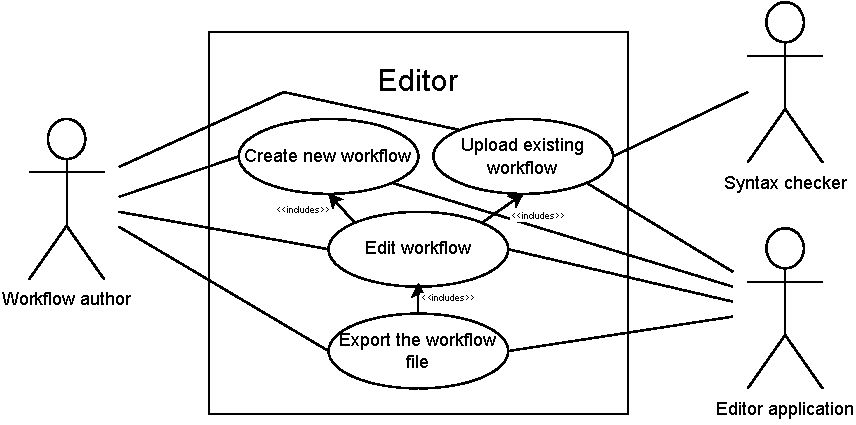
\includegraphics{./img/editorUC.pdf}
    \caption{Editor - Use Case UML diagram}
\end{figure}

% \begin{figure}[h!]
%     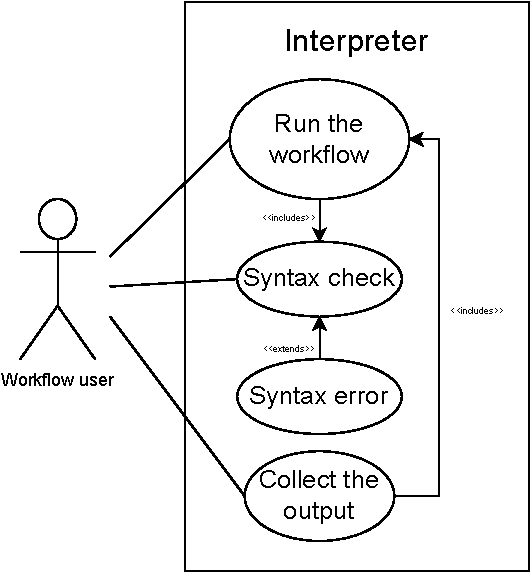
\includegraphics{./img/interpreterUC.pdf}
%     \caption{Interpreter - Use Case UML diagram}
% \end{figure}


\defcitealias{PPatch21}{PPatch21}
\defcitealias{PReadme22}{PReadme22}

\section*{Related Work}
As of now, there are already numerous solutions for automating web actions on the market. 
A majority of those uses existing web browsers and offer a programmable interface for simulating user input.

\textbf{Cypress} is a \ac{E2E} Javascript testing framework containing various assertions for \ac{QA} testing of webpages.
It supports multiple web browsers and offers its own UI and toolkit for test programming and running. 
Due to its strong orientation towards testing, it does not provide much methods for data extraction and crawling.

\textbf{Selenium WebDriver} is a fairly popular tool among web UI testers, as it offers a wide variety of methods for \ac{QA} testing.
Distributed as a multilanguage library, Selenium implements a high-level interface for controlling web browsers from code.
% Aside from regular commercial web browsers, Selenium also implements interfaces for PhantomJS and HTMLUnit, both headless scriptable browsers used as a lightweight alternative to regular browsers.

\textbf{Puppeteer} is a low-level library used for web browser automation. 
Unlike Cypress and Selenium, Puppeteer supports Chrome (or Chromium) as its only backend browser as of now (\today).

The communication with the browser is implemented via WebSockets and the DevTools Protocol, a Chromium-specific set of commands.
This allows Puppeteer to exceed Selenium both in stability and performance, sporting up to $17\%$ speedup in benchmarks \citepalias{Chck21}.

\textbf{Playwright} is another low-level library multilanguage library offering programmable ways of controlling web browser.
For browser communication, Playwright uses similiar technology as Puppeteer, unlike Puppeteer, Playwright supports multiple commercial browsers (Chromium, Firefox, Webkit as of \today).

Due to differences between browsers and partial incompatibility of protocols, Playwright is distributed with patched versions of Firefox and Webkit \citepalias{PPatch21}.
Stock versions of Chromium based browsers (Google Chrome, Microsoft Edge) are supported. \citepalias{PReadme22}

\vspace{\baselineskip}

All the aforementioned examples however require programming, which can mean a significant barrier to entry for beginners.

